\chapter{Protokolle Lichttechnik}
\lhead{Kapitel 2: \emph{Protokolle Lichttechnik}}

In der Lichttechnik haben sich mehrere Standards durchgesetzt. Abhängig vom Anwendungsfall werden meistens verschiedene Standards bevorzugt. Bei der Gebäudebeleuchtung wird DALI häufig genutzt. Aber auch neuere Technologien wie z.B. ZigBee oder Philips Hue setzten sich bei der privaten SmartHome Integration durch. In der Bühnentechnik hat sich der DMX Standard als industrieller Standard durchgesetzt. Der DMX Standard ist ebenfalls offen und kann von jedem implementiert werden. Allerdings sind die Leuchten, die auf dem freien Markt erhältlich sind, oft teuer.  Für die Signalsteuerung ist entweder ein DMX Controller oder DMX Software erforderlich. Auch diese sind oft teuer  oder lizenzpflichtig. In der Hobbyszene wird daher gerne ein anderes Protokoll für die Lichtkoordination umfunktioniert: MIDI. Das Protokoll, wurde ursprünglich für die Übertragung von Musik erstellt, kann aber auch genutzt werden, um Lichtinformationen zu übermitteln.


\section{DALI}
% TODO wie sieht das Datenpaket von DALI aus? - werden jedes mal alle Information gesendet, oder ist es nur eventbasiert?
Das Lichtsteuerungsprotokoll DALI (\emph{Digital Addressable Lighting Interface}) ist in der Gebäudebeleuchtung weitverbreitet. Vor allem in Bürogebäuden, Hotels oder auch im Einzelhandel wird es oft verwendet. Einzelne Leuchten können spezifisch gesteuert oder zu Gruppen zusammengefasst werden.

DALI wurde erstmals in den späten 1990er \cite{DALI-2_certification} von der europäischen Lichtindustrie entworfen. Viele Hersteller verwenden seither das Protokoll weltweit für die Steuerung von deren Produkten. Dadurch können Vorschaltgeräte vor den Leuchten von verschiedenen Hersteller nebeneinander eingesetzt werden, ohne dass der Anwender sich mit technischen Unterschieden auseinandersetzten muss \cite[S.2, ch. 3.1]{DALI-Lichtmanagement}.

Eines der Hauptvorteile von DALI ist die genaue Steuerung einzelner oder zu Gruppen zusammengefassten Leuchten. Jede Leuchte kann eine eindeutige Adresse zugewiesen bekommen. Die einzelnen Leuchten können dadurch separat voneinander gesteuert werden. Das Protokoll ermöglicht es, die Leuchten zu dimmen und somit maßgeschneidert an die speziellen Bedürfnisse der Umgebung anzupassen. Helles Arbeitslicht, Umgebungslicht als auch eine Akzentbeleuchtung kann damit gesteuert werden. Es können auch verschiedene Lichtszenen vorprogrammiert werden, z.B. eine Szene für die Tag- und Nachtbeleuchtung, (vgl.\ref{fig:dali_scenes}).

\begin{figure}[H]
	\centering
	\begin{subfigure}{.5\textwidth}
		\centering
		\shadowimage[width=.6\linewidth]{Pictures/DaliSchauraumTag}
		\caption{Szene Schauraum Tag}
	\end{subfigure}%
	\begin{subfigure}{.5\textwidth}
		\centering
		\shadowimage[width=.6\linewidth]{Pictures/DaliSchauraumNacht}
		\caption{Szene Schauraum Nacht}
	\end{subfigure}
	\caption{Beispiele für Lichtszenen \cite[S.6]{DALI_Handbuch}}
	\label{fig:dali_scenes}
\end{figure}

DALI ist ein digitales Protokoll, welches eine bidirektionale Kommunikation zwischen Leuchten und Controller ermöglicht\cite[S.1]{DALI-Lichtmanagement}. Dadurch können auch Fehlermeldungen der Leuchten ausgelesen werden. Eine kaputte Leuchte kann so einfach gefunden und ausgetauscht werden.  Aber auch andere Sensoren wie Tageslichtsensoren oder Bewegungssensoren können ins Netzwerk eingeschlossen werden. Damit kann die Helligkeit beispielsweise durch das Tageslicht oder durch die Anwesenheit von Menschen gesteuert werden. Der Stromverbrauch kann so massiv reduziert werden, da die Leuchten nur benutzt werden, wenn sie auch tatsächlich gebraucht werden.

DALI basiert auf einem einfachen zwei Kabel Bussystem. Das Bussystem kann am Ende des Busses fortgeführt werden, um es nachträglich zu erweitern. Der DALI Bus besteht aus zwei Leitungen. Ist die Verwendung von DALI gewünscht, so müssen ggf. diese Leitungen nachgerüstet werden. Wird dies bereits beim Bau eingeplant, können die freien Adern in einer Netzleitung benutzt werden\cite[S. c.3.2.2]{DALI-Lichtmanagement} (vgl.\ref{fig:wiring diagram}). Auf die Polarität der DALI Signale muss nicht geachtet werden \cite[p.3]{DALI_Handbuch}.

\begin{figure}[H]
	\centering
	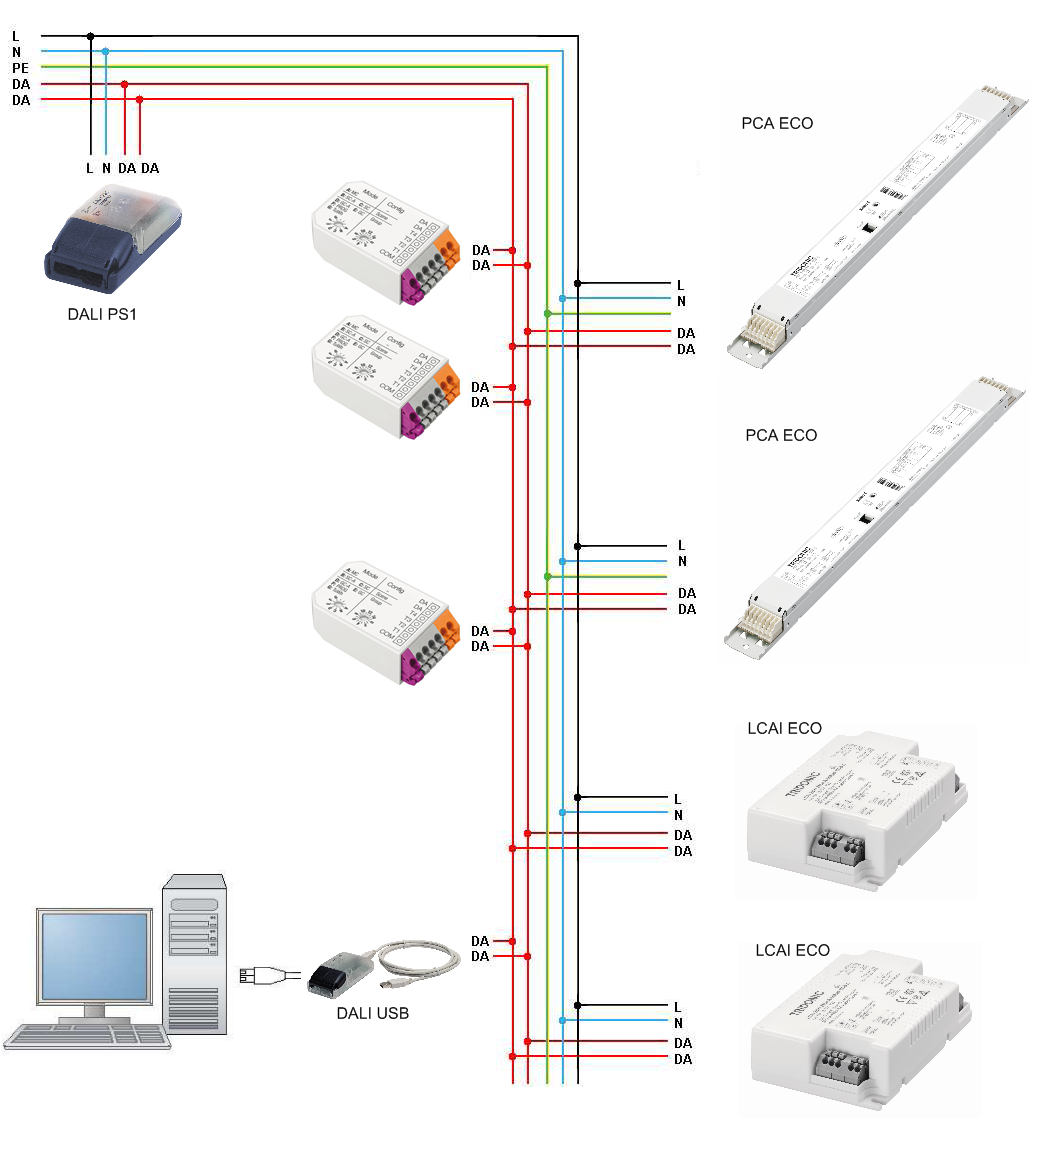
\includegraphics[width=.6\linewidth]{Pictures/DaliInstallation}
	\caption{Verdrahtungsdiagramm \cite[S.64]{DALI_Handbuch}}
	\label{fig:wiring diagram}
\end{figure}

Weiterhin können die DALI Controller einfach programmiert werden, um eine spätere Änderung der Leuchten einzustellen.

Neben den vielen Vorteilen hat das DALI Protokoll auch einige Limitierungen. Ein DALI Bus ist insgesamt auf maximal 64 Adressen begrenzt \cite[S.7]{DALI_Handbuch}. Jede Adresse hat einen Wertebereich von 8 Bit \cite[S.1]{DALI-Lichtmanagement}. Eine Leuchte kann daher z.B. auf maximal 256 verschiedene Helligkeitsstufen eingestellt werden. Es können maximal 16 Gruppen und 16 verschiedene Lichtszenen programmiert werden. Die geringe Datenrate von $1,2 \frac{\SI{}{\kilo\bit}}{\SI{}{\s}}$ limitiert das Protokoll auf eine Aktualisierungsrate von ca. 25-30 Herz. Weiterhin können die Kabel maximal 300 Meter lang verlegt werden, bevor sie wieder verstärkt werden müssen \cite[S.3]{DALI_Handbuch}. 

Im Vergleich zu einem analogen System, hat DALI keine großen Probleme mit Interferenzen oder Störungen von externen Quellen. Das Protokoll ist selbst auf langen Strecken sehr zuverlässig.

Insgesamt ist DALI ein leistungsstarkes Lichtsteuerprotokoll, das durch seine Flexibilität, Genauigkeit und Energieeffizienz viele Vorteile gegenüber einem analogen traditionellen Steuersystem bietet. Die Adaption der Lichtindustrie hat es zu einem Industriestandard für die Gebäudebeleuchtung aller Art gemacht.

\section{DMX}

DMX (\emph{Digital Multiplex}) ist ebenfalls wie DALI ein Lichtsteuerprotokoll. Der Anwendungsfall ist meist jedoch ein anderer. DMX ist der Industriestandard in der Bühnentechnik und Unterhaltungsindustrie. DMX wird benutzt, um steuerbare Leuchten zu koordinieren, wie z.B. bewegbare Leuchten und LED Farbleuchten. Dabei können alle Leuchten zentral von einem dedizierten physischen Controller oder über Software gesteuert werden (vgl. \ref{fig:dmx_use_example}).


\begin{figure}[H]
	\centering
	\shadowimage[width=0.5\linewidth]{Pictures/dmxInstallation}
	\caption{DMX gesteuerte Lichtszene in einer Berliner Bar}
	\label{fig:dmx_use_example}
\end{figure}


DMX wurde erstmals im Jahr 1986 vorgestellt \cite[S.5, ch. 2.1]{DMX101-Handbook}. Seither wurde es der verbreitetste Industriestandard für koordinierte Lichtshows. Genau wie DALI, ist DMX ebenfalls ein digitales Steuerprotokoll. Über ein DMX Kabel kann jeweils ein DMX Universum übertragen werden. Ein DMX Universum kann mehrere Kanäle gleichzeitig steuern. Ein Kanal kann dabei, z.B. auf die Farbe einer Leuchte, oder die Helligkeit einer Leuchte abgebildet werden. Das DMX Protokoll basiert auf einer seriellen Datenübertragung. Das Protokoll baut auf dem RS-485 Standard\cite[S.11, ch. 3.2]{DMX101-Handbook} auf.

Eines der Hauptvorteile von DMX ist die zentrale Steuerung von einer großen Anzahl von Leuchten über eine Konsole. Komplexere Leuchtkonstellationen mit vielen unterschiedlichen Leuchten sind dadurch umsetzbar. Mehrere Leuchten können so zusammengeschaltet werden, um komplizierte Effekte und Lichtszenen aufzubauen. Oftmals werden verschiedene Animationsmuster vorprogrammiert und als Lichtsequenz abgespeichert. Lichtgestalter/-innen können dadurch einfach und schnell verschiedene Animationen und Konfigurationen aufrufen, um die Lichtszenerie auf die verschiedenen Phasen der Show abzustimmen.

Die Verkabelung von DMX ist einfach. In der Regel wird das Datensignal getrennt von der Stromversorgung geführt. Das Datensignal kann mithilfe einer Gänseblümchenkette (\emph{Daisy Chain}) (vgl. \ref{fig:dmx_wiring diagram}), einfach von Leuchte zu Leuchte verkabelt werden. Am Ende der Gänseblümchenkette, ist ein DMX-Terminator erforderlich, um die Datenintegrität innerhalb des Busses zu gewährleisten. Bei größeren Distanzen (ab 300 Meter) muss das DMX Signal verstärkt werden, um eine sichere Datenübertragung zu gewährleisten.

\begin{figure}[H]
	\centering
	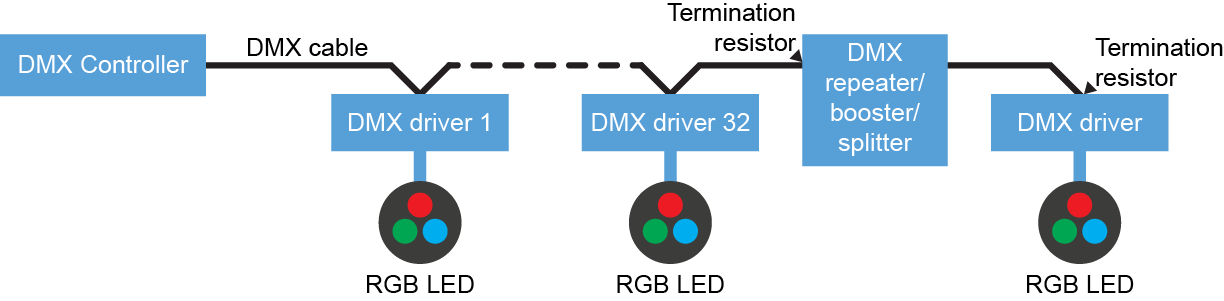
\includegraphics[width=.9\linewidth]{Pictures/dmxWiringDiagram}
	\caption{Verdrahtungsdiagramm \cite[S.64]{DMX_Wiring}}
	\label{fig:dmx_wiring diagram}
\end{figure}

DMX ist unter anderem auch sehr flexibel und konfigurierbar. Das Protokoll erlaubt die Ansteuerung von selbst gebauten Leuchten. Hersteller können für ihre Produkte auch bereits vorgefertigte DMX Konfigurationen mitliefern. Lichtgestalter/-innen bekommen dadurch eine genaue Kontrolle über die Funktionalitäten der einzelenden Leuchten, wie z.B. die Farbeinstellungen oder Filterauswahl.

Ein weiterer Vorteil von DMX, ist die Möglichkeit mehrere Systeme zusammenzuschalten. Eine große Anzahl an DMX Universen können über eine Konsole gesteuert werden, um eine größere Anzahl von Leuchten zu steuern. DMX kann auch mit Audio oder Video Systemen integriert werden, um eine synchrone Licht und Sound Show mit visuellen Effekten aufzubauen.

Neben den vielen Vorteilen hat DMX auch einige Einschränkungen. Ein unverstärktes Signal kann maximal 300 Meter lang werden, bevor das Signal durch die Signalverschlechterung erneut verstärkt werden muss. Daher müssen für längere Strecken zwingend DMX Verstärker verwendet werden, um die Signalstärke beizubehalten. Ein DMX Universum erlaubt eine Kontrolle von bis zu 512 Kanälen. Die Datenpakete werden mit einer Datenrate von insgesamt $250 \frac{\SI{}{\kilo\bit}}{\SI{}{\s}}$ gesendet. Sind alle Kanäle ausgeschöpft, ist die maximale Aktualisierungsrate $44 \frac{\SI{}{Aktualisierungen}}{\SI{}{\s}}$ \cite[S.18, table6]{DMX512-Protocol-Standard}

Zusammengefasst ist das DMX Protokoll ein verbreitetes Lichtsteuerungsprotokoll, welches in der Industrie oft zu finden ist. Die Möglichkeit mehrere Leuchten getrennt voneinander ansteuern zu können, und die Integrierbarkeit mit anderen Systemen, hat es zu einer wesentlichen Komponente für Lichtgestalter/-innen gemacht.


\section{MIDI}
%TODO optional: maybe talk about a bit about midi 2.0

Das MIDI (\emph{Musical Instrument Digital Interface}) Protokoll ist ein Musikprotokoll, welches primär in der Musikszene genutzt wird. MIDI erlaubt es elektronische Musikinstrumente, Computer, oder auch andere Geräte wie z.B. Synthesizer, miteinander zu verknüpfen. Musizierende können dadurch den Sound eines Instrumentes während des Spielens anpassen, und neue Effekte auf kreative Art und Weise aufbauen.

MIDI wurde zuerst in den frühen 1980er Jahren \cite[S.1]{MIDI-Complete-SPECIFICATION} vorgestellt, und hat sich schnell als neuer Standard für die elektronische Musikproduktion durchgesetzt. Das Protokoll erlaubt eine Übertragung von musikalischen Daten, wie Ton-An, Ton-Aus, Tonhöhe, Dämpfung, Modulation etc. zwischen MIDI-Kompatiblen Geräten \cite[S.9]{MIDI-DETAILED-SPECIFICATION}. Dadurch können Künstler/-innen Musik mit einem elektronischen Klavier aufnehmen und die Töne, zusammen mit Metainformationen, wie dem Tastendruck, Dauer des Tastenanschlages usw. aufnehmen, und auf einem anderen Gerät abspielen oder auch im Nachhinein verändern. 

MIDI kann auch benutzt werden, um virtuelle Instrumente zu simulieren und diese klanglich mit Software Erweiterungen stark zu verändern. Künstler/-innen haben dadurch eine Vielzahl von verschieden Geräuschen und Effekten zur Auswahl.

Ein weiterer Vorteil des MIDI Protokolls ist die große Anzahl von MIDI kompatiblen Geräten. MIDI kompatible Geräte sind unter anderem elektronische Tasteninstrumente, Synthesizer, Trommelmaschinen und viele weitere. Künstler/-innen können einfach eine Vielfalt von Geräten zusammen benutzen, um neue kreative und raffinierte musikalische Werke zu produzieren.

Im Vergleich zu DMX werden die Daten im MIDI Protokoll auf einer anderen Art und Weise verschickt. DMX sendet jedes Mal alle aktiven Kanäle. Sollte ein Paket nicht beim Empfänger ankommen, ist dies kein Problem, da das nächste Paket wieder alle Informationen enthält. Dadurch werden Informationen, die sich nicht ändern, jedes Mal neu versendet.

Bei MIDI werden nicht kontinuierlich alle Informationen gesendet. MIDI hat einen anderen Ansatz. Signale, wie z.B. Ton-An beim Tastenanschlag, werden nur einmal gesendet \cite[S.3]{MIDI-DETAILED-SPECIFICATION}. Dadurch werden keine Informationen redundant versendet.

Das MIDI Protokoll wurde erweitert, um neben den Musikinformationen, zusätzlich auch Lichtinformationen versenden zu können, \cite[S.1]{MIDI-Visual-Control} (vgl.\ref{fig:Midi_Light_Integration}). Die Leuchten, können programmiert werden, um auf Ton-An und Ton-Aus Signale zu hören \cite[S.4]{MIDI-Visual-Control}. Auch über \emph{Control Change} Signale können Farben und weitere Optionen eingestellt werden \cite[S.6, ch. 2.2.1.2]{MIDI-Visual-Control}. 

\begin{figure}[H]
	\centering
	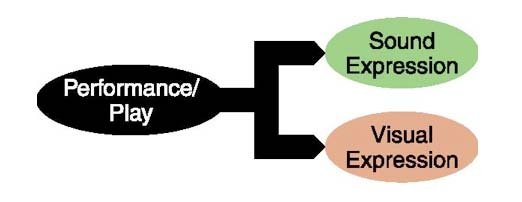
\includegraphics[width=.6\linewidth]{Pictures/MidiVisual}
	\caption{MIDI Licht Integration \cite[S. 1]{MIDI-Visual-Control}}
	\label{fig:Midi_Light_Integration}
\end{figure}

Die folgende Abbildung \ref{fig:MidiUseCase} zeigt ein selbstgebautes Steuergerät, welches Leuchten mithilfe eines MIDI Eingangssignales steuert.
\begin{figure}[H]
	\centering
	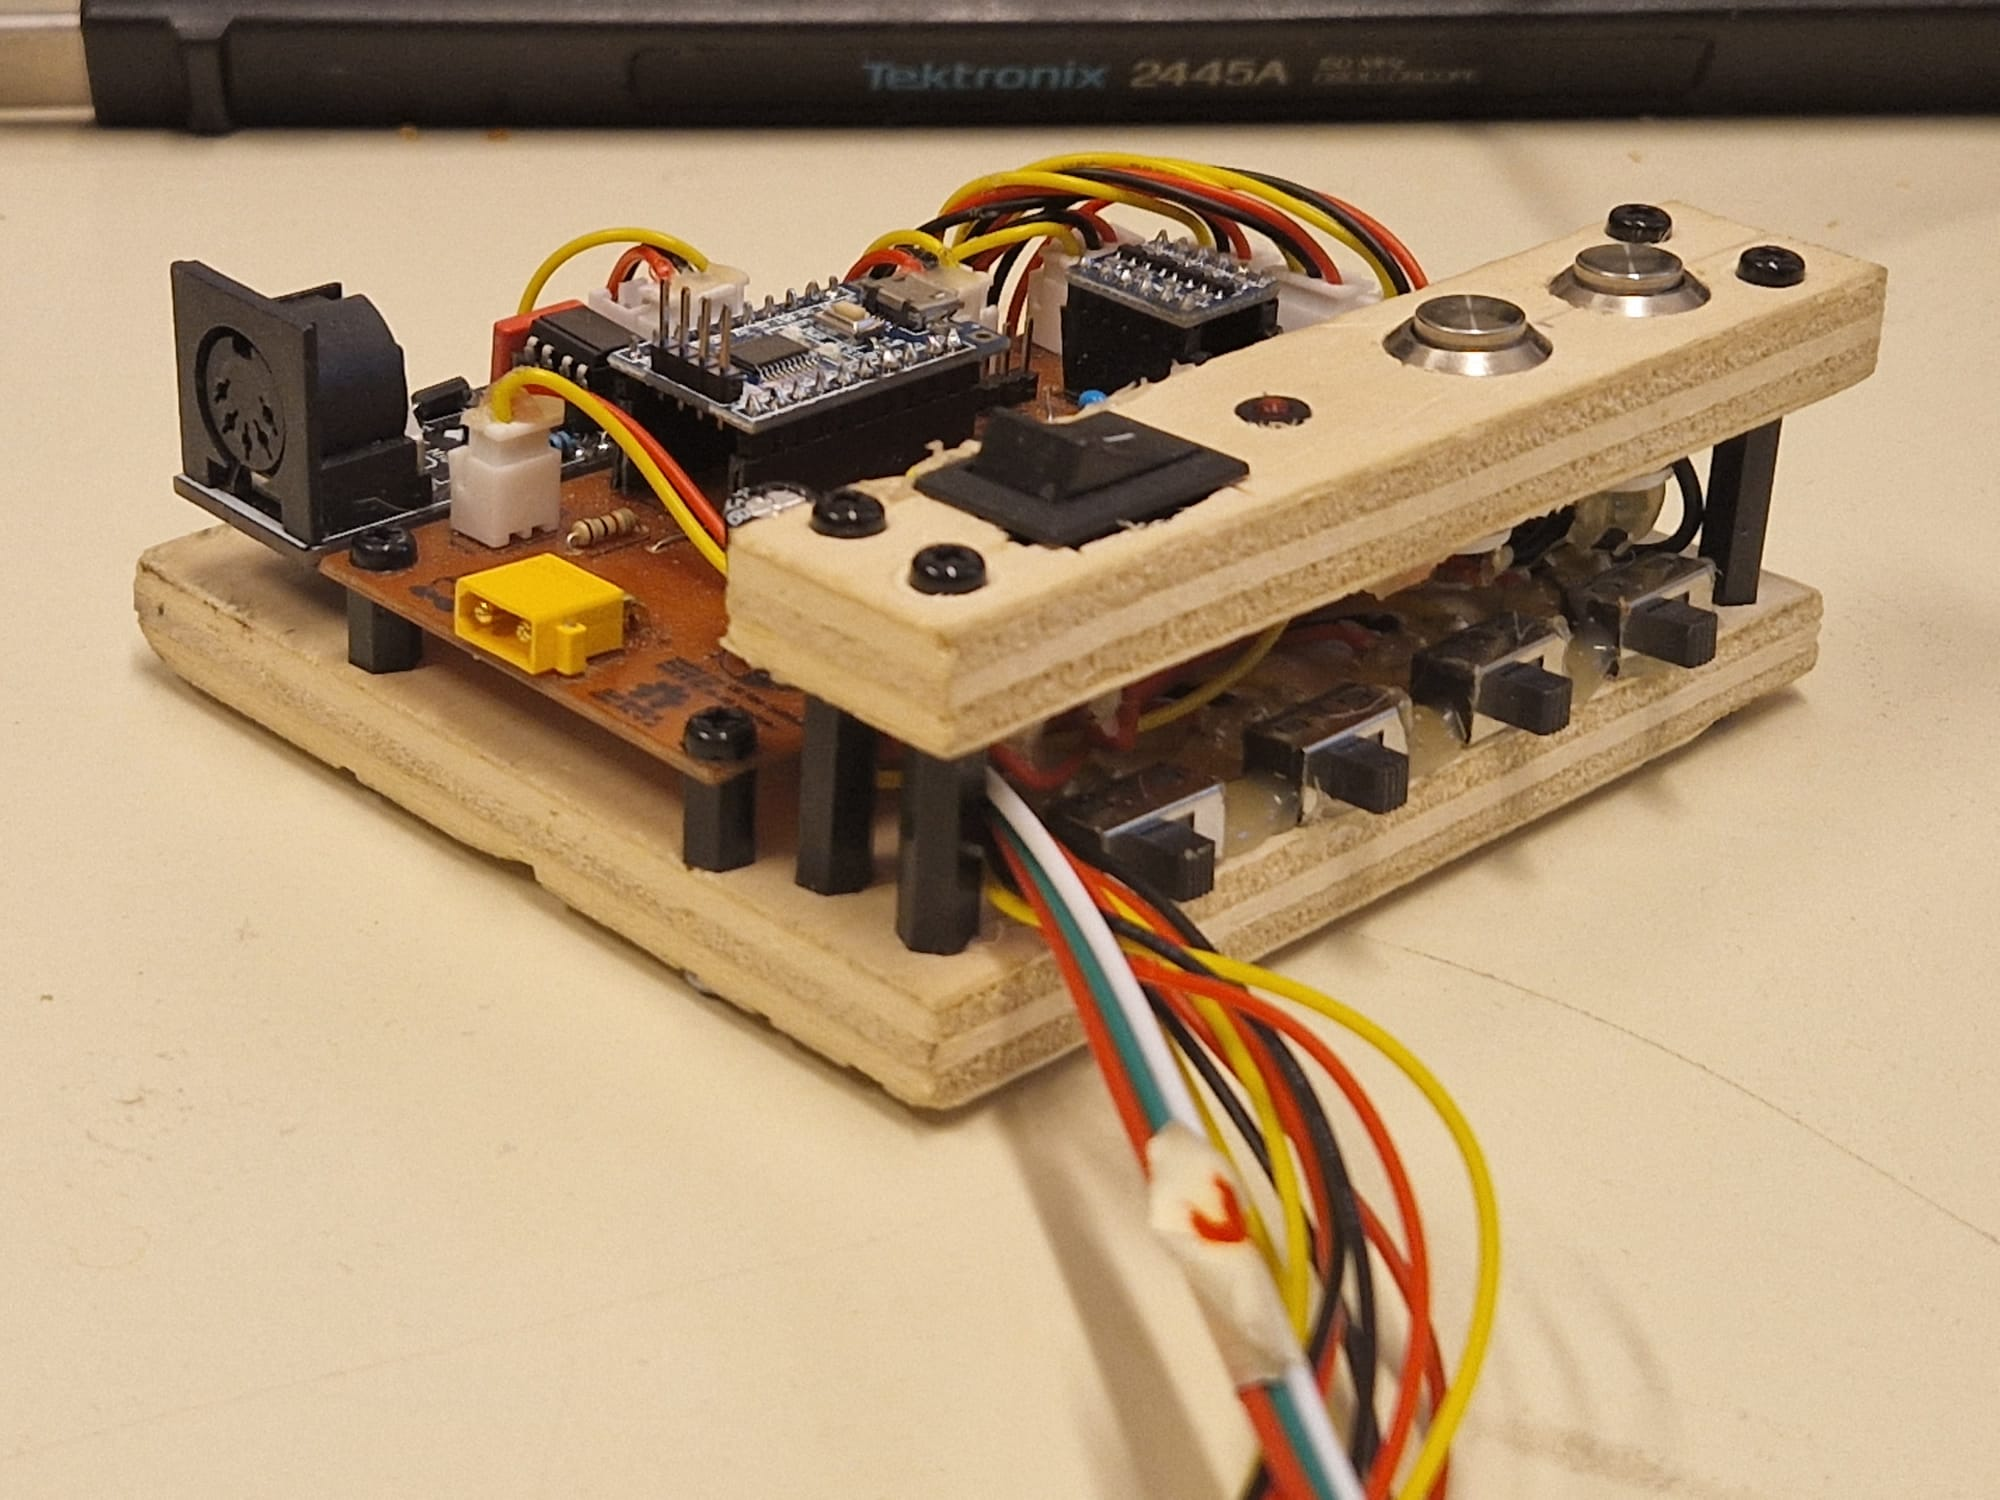
\includegraphics[width=.5\linewidth]{Pictures/midiUseCase}
	\caption{MIDI Steuergerät für Leuchten}
	\label{fig:MidiUseCase}
\end{figure}
 

Neben den vielen Vorteilen hat MIDI aber auch einige Einschränkungen. MIDI ist nicht in der Lage, rohe Audiodateien zu versenden. MIDI kann nur digitale Signale verschicken, welche die Parameter und Benutzung der Musikinstrumente beschreibt. Daher ist auch ein separates Audiosignal erforderlich, um die Musik aufzunehmen, die mithilfe von MIDI erstellt wird. MIDI läuft mit ca. $31 \frac{\SI{}{\kilo\bit}}{\SI{}{\s}}$ \cite[S. 1]{MIDI-DETAILED-SPECIFICATION}. DMX hat im Vergleich dazu eine 8-mal höhere Datenrate. 

Die genaue und flexible Einstellungen hat es für Musizierende eine wesentliche Komponente für die Musikproduktion gemacht.


\section{ZigBee}
% TODO optional: maybe include matter(application layer) (thread is physical layer)? its a IOT protocol
ZigBee ist ein Kabelloses-Protokoll, welches in den letzten Jahren stark an Popularität gewonnen hat. Es wird gerne für intelligente Wohnungen mit automatischem Licht etc. eingesetzt. Philips Hue ist eine Smarthome Produktgruppe, welche über das ZigBee Protokoll läuft, um Benutzer/-innen die Steuerung von Leuchten z.B. in einer Wohnung über das Mobiltelefon zu ermöglichen. Auch eine Integration mit anderen Systemen ist möglich. So kann das Lichtbild an die Musik angepasst werden, oder Jalousien, am Abend automatisch heruntergefahren werden. Das folgende Bild stellt eine exemplarische Verwendung von Philips Hue in einer Wohnung dar.

\begin{figure}[H]
	\centering
	\shadowimage[width=.5\linewidth]{Pictures/phillipsUseCase}
	\caption{Intelligente Wohnung mit  Philips Hue}
\end{figure}


ZigBee und IEEE 802.15.4 sind standardisierte Protokolle, welche die Netzwerkinfrastruktur bereitstellen. Dabei definiert der IEEE 802.15.4 Standard die physikalische Schicht, inklusive der MAC Adressen. ZigBee hingegen definiert die Netzwerk- und Anwendungsschicht \cite[S.5]{GettingStartedWithZigBee}.

ZigBee hat einen geringen Stromverbrauch mit entsprechend verlangsamten Datenraten. Dadurch können auch batteriebetriebene Produkte lange durchhalten. Das Protokoll wurde entwickelt, um mit allen möglichen IoT (\emph{Internet of Things}) Geräten zu kommunizieren.

ZigBee Geräte kommunizieren über eine Mesh-Netzwerk-Topologie \cite[S.10]{GettingStartedWithZigBee}. Das bedeutet, jedes Gerät (oder auch jeder Knotenpunkt) kann als Verstärker fungieren, um die Netzwerkreichweite zu vergrößern. Dadurch können ZigBee Geräte durch die Wohnung verteilt werden, um ein robustes und zuverlässiges System aufzubauen.

Philips Hue ist ein Produkt, welches sich auf inteligenten LED Leuchten fokussiert. Es kann auch mit anderen ZigBee kompatiblen Geräten verschaltet werden. Philips Hue kann per App einfach übers Mobiltelefon gesteuert werden. Die Helligkeit, Farbwärme oder auch ein Flackern wie bei einer Kerze kann eingestellt werden. Philips Hue kann unter anderem auch über Sprachassistenten wie Alexa oder dem Google Assistenten gesteuert werden.

Ein weiterer Vorteil vom Hue System, ist der einfache Aufbau und Einrichtung. Mithilfe der Hue App können Lichtszenen einfach erstellt und abgerufen werden. Zeitsysteme können einprogrammiert werden, und mit einer Internetverbindung von überall, auch außer Hause, ferngesteuert werden. Auch können Bewegungsmelder, Dimmer oder Batterie betriebene Schalter benutzt werden und überall im Hause verteilt werden, um die Lichter entspannt von überall aus steuern zu können. Auch intelligente Steckdosen können mit dem System kontrolliert werden. 

Die Frequenzbänder des ZigBee Protokolls überlappen sich mit den Frequenzbänden des Bluetooth und WLAN Standards (vgl.\ref{fig:ZigBee_Frequency_bands}).
\begin{figure}[H]
	\centering
	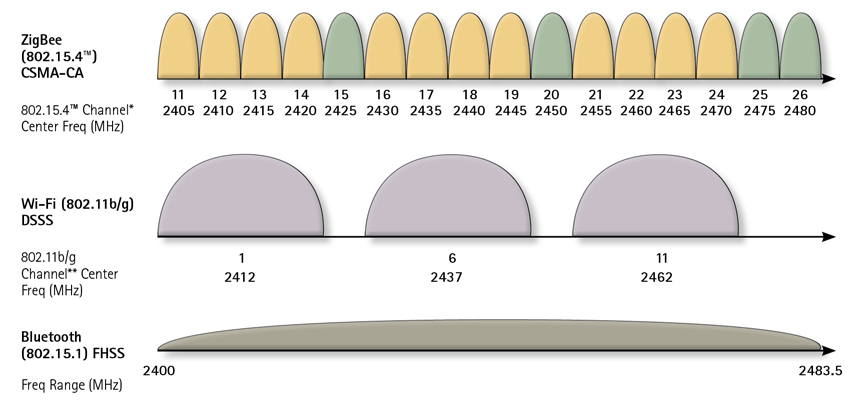
\includegraphics[width=.8\linewidth]{Pictures/ZigBeeRfOverlap}
	\caption{ZigBee Frequenzüberlappung \cite[S.23]{GettingStartedWithZigBee}}
	\label{fig:ZigBee_Frequency_bands}
\end{figure}
Die grauen Bänder haben weniger Überlappungen mit den WLAN-Kanälen. Sie können gewählt werden, um weniger Interferenzen zwischen den beiden Protokollen zu erhalten.

Durch die kabellose Kommunikation ist keine Nachrüstung von Kabelsystemen erforderlich. Dies erleichtert den Einstieg für Konsument/-innen erheblich. Sie müssen keine neuen Kabel verlegen, oder sich mit der Elektronik auskennen. ZigBee ist ein allgemeines Protokoll, welches für IoT Geräte aller Art entwickelt worden ist. Es wird oft bei Lichtinstallationen in privaten Wohnungen genutzt.

Zusammengefasst hat das ZigBee Protokoll und die Philipps Hue Produkte eine neue Nische im vernetzten und intelligenten Zuhause gefunden. Vor allem die einfache Installation und Nachrüstung macht es für den Verbraucher/-innen sehr einfach, auf Philips Hue umzuwechseln.

\section{Vergleich}

Die nachfolgende Tabelle \ref{tab:LightProtokollComparison} stellt die bereits angesprochenen Eigenschaften der Protokolle anschaulich da.

\begin{table}[H]
	\centering
	\resizebox{\textwidth}{!}{ %
		\begin{tabular}{ |c|c|c|c|c| } 
			\hline
			Kategorie / Protokoll & DALI & DMX & MIDI & ZigBee \\
			\hline
			Aktualisierungsrate & 30 Hz & 44 Hz & Signal basiert & Netzwerk abhängig \\
			Datenrate in $\frac{\SI{}{\kilo\bit}}{\SI{}{\s}}$ & 1,2  & 250 & 31.25 & 40 - 250 \\
			Unterschiedliche Kanäle & 64 Adressen & 512 Kanäle & 16 Geräte &  65,534 Geräte\\
			Topologie & Bus & Bus & Bus & Mesh (\emph{Peer-To-Peer}) \\
			Exemplarische Verwendung & Häuser & Bühnen & Hobby-/ Musikszene & Intelligentes Zuhause \\
			\hline
	\end{tabular}}
	\caption{Lichtsteuer Protokolle im Vergleich}
	\label{tab:LightProtokollComparison}
\end{table}
